\documentclass[notitlepage]{report}
\usepackage[margin=1in]{geometry}
\usepackage[utf8]{inputenc}
\usepackage{xcolor}
\usepackage{caption}
\usepackage{hyperref}
\usepackage{graphicx}
\usepackage{babel,blindtext}
\usepackage{subcaption}
\usepackage{hyperref}
\usepackage{multicol}
\setlength{\columnseprule}{1pt}
\usepackage{listings}
\usepackage{pgfplots}

\def\columnseprulecolor{\color{brown}}
\graphicspath{ {images/} }
%\usepackage{flafter}

\title{\Huge{COP290 Lab-2 Report}}
\author{
  Amaiya Singhal\\
  \texttt{2021CS50598}
  \and
  Sarwagya Prasad\\
  \texttt{2021CS10639}
  \and
  Om Dehlan\\
  \texttt{2021CS10076}
}
\date{}

\begin{document}
\maketitle

\section*{PART 2}
\subsection*{Testing}
To run and check each component of our project, we have made a \texttt{makefile} which compiles the needed source files, create an executable file and then runs it.

\begin{figure}[hbp]
    \centering
    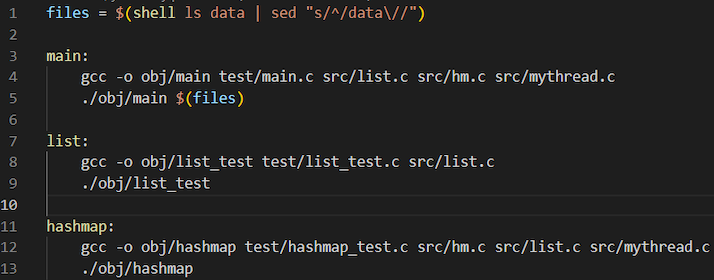
\includegraphics[width = 1\linewidth]{makefile_code.png}
    \caption*{The makefile}
\end{figure}
\begin{itemize}
    \item \texttt{make list} and \texttt{make hashmap} run the list and hashmap test files respectively.
    \item \texttt{make main} runs the main test file, with all the files present in \texttt{data} directory as arguments.
\end{itemize}

\pagebreak

\subsection*{Checkpoint 1}
\subsubsection*{Testing Hashmap in \texttt{hashmap\textunderscore test.c}}
After completing the code for the hashmap (\texttt{hm.c}), we tested it on the provided test file – \texttt{hashmap\textunderscore test.c} and got the following output:

\begin{figure}[hbp]
    \centering
    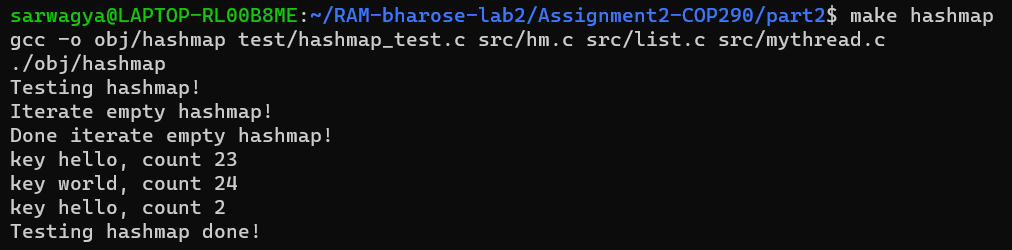
\includegraphics[width = 1\linewidth]{hashmap_test_out.png}
    \caption*{Output of \texttt{hashmap\textunderscore test.c}}
\end{figure}

\noindent This is the expected output. Thus we were convinced that each individual function in \texttt{hm.c} works correctly. 
\newline
\newline
\subsubsection*{Testing Hashmap in \texttt{main.c}}
\noindent Next we ran the file on \texttt{main.c} by commenting out thread related commands and replacing them with a direct call of the function \texttt{readFile()} on the 4 .txt files provided in the \texttt{data/} directory.

\begin{figure}[hbp]
    \centering
    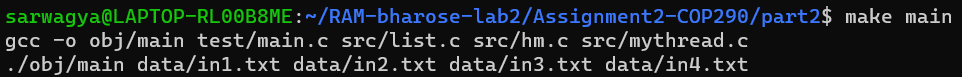
\includegraphics[width = 1\linewidth]{checkpoint1_command.png}
    \caption*{command}
\end{figure}

\begin{figure}[hbp]
    \centering
    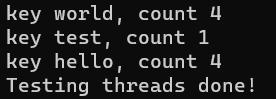
\includegraphics[width = 0.35\linewidth]{checkpoint1_out.png}
    \caption*{Hashmap Values}
\end{figure}

\noindent This is the expected output confirming the correctness of the implemented hashmap.

\pagebreak
\subsection*{Checkpoint 2}
\subsubsection*{Concurrency with threads}

\noindent Firstly we implemented the functions \texttt{mythread\textunderscore init}, \texttt{mythread\textunderscore create} and \texttt{mythread\textunderscore join} in \texttt{mythread.c}. 
\newline
\newline
\noindent After commenting out lines relating to \texttt{mythread\textunderscore yield}, \texttt{acquire\textunderscore bucket} and \texttt{release\textunderscore bucket}, we ran the \texttt{main} file on the 4 .txt files provided, the correct output was obtained.

\begin{figure}[hbp]
    \centering
    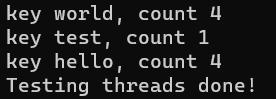
\includegraphics[width = 0.35\linewidth]{checkpoint1_out.png}
    \caption*{Hashmap Values}
\end{figure}

\noindent This output matches the output obtained from the single thread program in Checkpoint 1.

\subsection*{Checkpoint 3}
\subsubsection*{Locks}
\noindent In this case each thread ran individually and only switched to the next thread once the previous one was completed.
\newline
\newline
\noindent Next we implemented \texttt{mythread\textunderscore yield} so that the threads could run concurrently. 
\newline
\newline
\noindent After commenting code related to \texttt{acquire\textunderscore bucket} and \texttt{release\textunderscore bucket}, we ran the \texttt{main} file and got the following output: 

\begin{figure}[hbp]
    \centering
    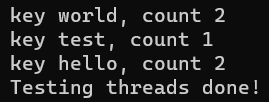
\includegraphics[width = 0.35\linewidth]{checpoint3_wrongOut_1.png}
    \caption*{Hashmap Values}
\end{figure}

\noindent Clearly, this output was wrong as it reports less frequency of the words. 
\newline
\newline
\noindent We also checked the code for a set of files such that each file contained multiple occurrences of the same word., i.e. in1.txt contained only 5 \texttt{hello}, in2.txt only contained 3 \texttt{test} and in3.txt contained only 4 \texttt{world}, and obtained the correct output:

\begin{figure}[hbp]
    \centering
    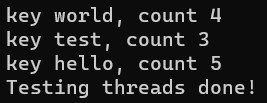
\includegraphics[width = 0.35\linewidth]{checpoint3_wrongOut_samewords.png}
    \caption*{Hashmap Values}
\end{figure}

\pagebreak
\subsubsection*{Race Condition}
\noindent Thus we could conclude that the threads were interfering with each other for access to the memory of each word in the hashmap, i.e., we were running into a \textbf{race condition} where different threads are trying to increment the same value, but read the same value rather than reading the value incremented by other threads. 
\newline
\noindent For example if thread 1 and thread 2 both read the word \textbf{hello}, they read the current frequency of hello in the hashmap, say 2, and each increment it to 3 and write it back. So we got an incorrect value of 3 as opposed to the correct value of 4. 
\newline
\newline
\noindent When we ran it on files containing only a single word, there was no chance of interfering as each thread utilized different memory and thus we obtained the correct output.

\subsubsection*{Solving the Race Condition}
To solve the race condition issue, we implemented \textbf{locks} which ensured that while one thread is working on a particular memory (in our case: one slot/bucket of the hashmap), other threads could not have access to it until the thread finishes. 
\newline
\newline
\noindent After implementing \texttt{acquire\textunderscore bucket} and \texttt{release\textunderscore bucket}, we ran the main code to get:

\begin{figure}[hbp]
    \centering
    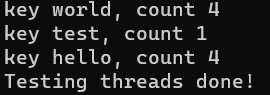
\includegraphics[width = 0.35\linewidth]{checkpoint3_withBucket.png}
    \caption*{Hashmap Values}
\end{figure}
\noindent which was the expected correct output. Thus, we had resolved the race condition.

\pagebreak

\section*{PART 3}

Plotting from data:

\begin{multicols}{2}
\noindent \textbf{1. Different Files: }
 We observe that the time taken is more for Part 2 than Part 3. This is because Part 2 implements concurrency whereas Part 3 uses parallelism and takes advantage of the multiple cores of the system with multiple threads running at once. This reduces the running time.


\columnbreak
\begin{center}
\begin{tabular}{ |c|c|c| } 
\hline
 No. of Files & Part 2 & Part 3 \\
 \hline
 1 & 4.92915500 & 4.87719500\\ 
 2 & 14.08958100 & 10.62400800\\ 
 3 & 36.06447200 & 22.95074200\\ 
 4 & 80.11478500 & 51.09996900\\ 
 5 & 126.81183300 & 73.60158900\\ 
 6 & 200.98808500 & 108.03950900\\ 
 \hline
\end{tabular}
\end{center}

\centering
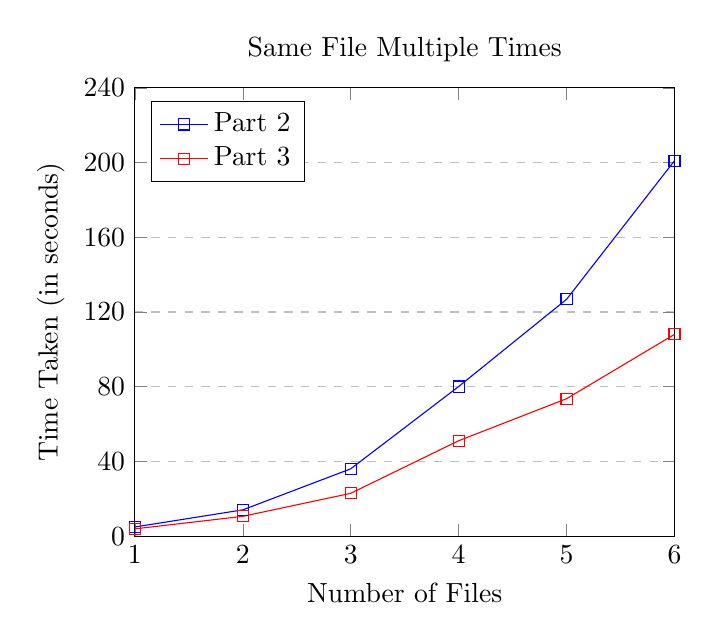
\begin{tikzpicture}
\begin{axis}[
    title={Same File Multiple Times},
    xlabel={Number of Files},
    ylabel={Time Taken (in seconds)},
    xmin=1, xmax=6,
    ymin=0, ymax=240,
    xtick={1,2,3,4,5,6},
    ytick={0,40, 80, 120, 160, 200, 240},
    legend pos=north west,
    ymajorgrids=true,
    grid style=dashed,
]

\addplot[
    color=blue,
    mark=square,
    ]
    coordinates {
    (1, 4.92915500)(2, 14.08958100)(3, 36.06447200)(4, 80.11478500)
    (5, 126.81183300)(6, 200.98808500)
    };

\addplot[
    color=red,
    mark=square,
    ]
    coordinates {
    (1, 3.92485800) (2, 10.62400800) (3, 22.95074200) (4, 51.09996900)
    (5, 73.60158900)(6, 108.03950900)
    };
    \legend{Part 2, Part 3}


\end{axis}
\end{tikzpicture}
\end{multicols}

\hrule
\begin{multicols}{2}
\noindent \textbf{2. Same file multiple times: }
 We observe that the times in Part 2 are more than Part 3 by a significant amount and this time is more than the first case where we ran different files. This is because running multiple instances of the same file will lead to multiple conflicts and hence increases the time significantly.


\columnbreak
\begin{center}
\begin{tabular}{ |c|c|c| } 
\hline
 No. of Files & Part 2 & Part 3 \\
 \hline
 1 & 4.87719500 & 3.97829800 \\ 
 2 & 21.06525300 & 15.80600400 \\ 
 3 & 52.61153600 & 36.81120600 \\ 
 4 & 103.78924800 & 65.79055500 \\ 
 \hline
\end{tabular}
\end{center}

\centering
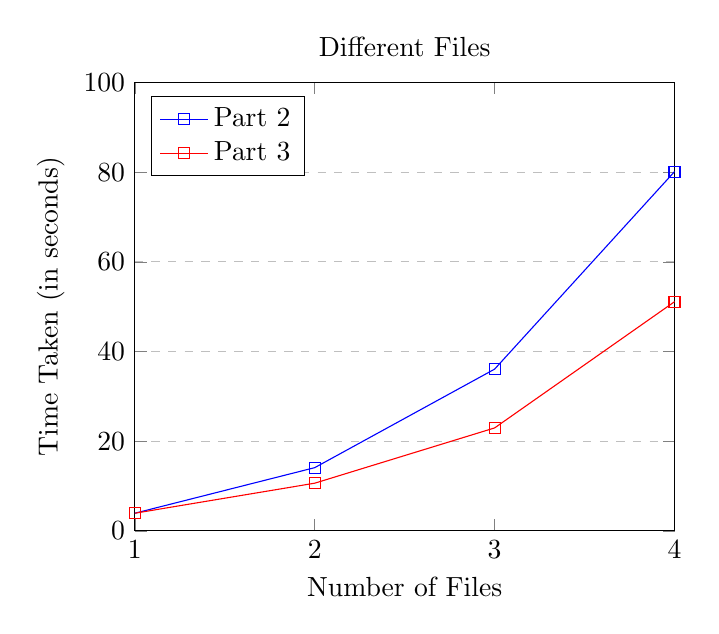
\begin{tikzpicture}
\begin{axis}[
    title={Different Files},
    xlabel={Number of Files},
    ylabel={Time Taken (in seconds)},
    xmin=1, xmax=4,
    ymin=0, ymax=100,
    xtick={1,2,3,4},
    ytick={0,20,40,60,80,100},
    legend pos=north west,
    ymajorgrids=true,
    grid style=dashed,
]

\addplot[
    color=blue,
    mark=square,
    ]
    coordinates {
    (1, 3.92485800) (2, 14.08958100) (3, 36.06447200) (4, 80.11478500) (5,126.81183300) (6,200.98808500)
    };

\addplot[
    color=red,
    mark=square,
    ]
    coordinates {
    (1, 3.92485800) (2, 10.62400800) (3, 22.95074200) (4, 51.09996900) (5,73.60158900) (6,108.03950900)
    };
    \legend{Part 2, Part 3}

\end{axis}
\end{tikzpicture}
\end{multicols}
\pagebreak

\begin{multicols}{2}
\noindent \textbf{3. One File of Increasing sizes: }
 We observe that the times in Part 2 are more than Part 3 but by a small amount. This is because since we are running on only 1 file, we do not take advantage of parallelism and hence the results in both the parts are comparable. The time is O($n^2$).


\columnbreak
\begin{center}
\begin{tabular}{ |c|c|c| } 
\hline
 No. of Files & Part 2 & Part 3 \\
 \hline
 1 & 4.87719500 & 3.97829800 \\ 
 2 & 21.06525300 & 15.80600400 \\ 
 3 & 52.61153600 & 36.81120600 \\ 
 4 & 103.78924800 & 65.79055500 \\ 
 \hline
\end{tabular}
\end{center}

\centering
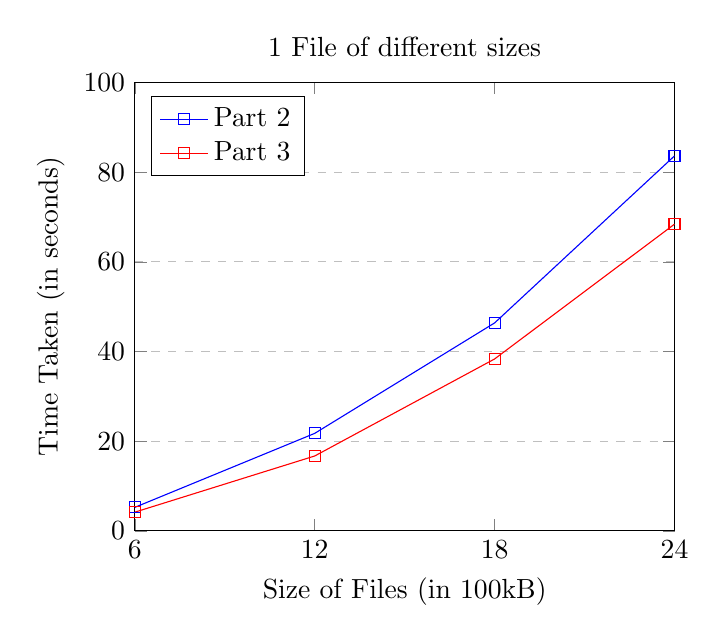
\begin{tikzpicture}
\begin{axis}[
    title={1 File of different sizes},
    xlabel={Size of Files (in 100kB)},
    ylabel={Time Taken (in seconds)},
    xmin=6, xmax=24,
    ymin=0, ymax=100,
    xtick={6,12,18,24},
    ytick={0,20,40,60,80,100},
    legend pos=north west,
    ymajorgrids=true,
    grid style=dashed,
]

\addplot[
    color=blue,
    mark=square,
    ]
    coordinates {
    (6, 5.23706200) (12, 21.73853300) (18, 46.37371000) (24, 83.62567000)
    };

\addplot[
    color=red,
    mark=square,
    ]
    coordinates {
    (6, 4.16374500) (12, 16.69273100) (18, 38.33668600) (24, 68.40319200)
    };
    \legend{Part 2, Part 3}
    
\end{axis}
\end{tikzpicture}
\end{multicols}

\hrule
\begin{multicols}{2}
\noindent \textbf{4. Files containing same word repeated times: }
 We observe that the times in Part 2 are almost the same as Part 3.


\columnbreak
\begin{center}
\begin{tabular}{ |c|c|c| } 
\hline
 No. of Files & Part 2 & Part 3 \\
 \hline
 1 & 43.50957600 & 35.80605200 \\ 
 2 & 86.80219800 & 80.46090200 \\ 
 3 & 130.90629800 & 127.08874900 \\ 
 4 & 179.70722000 & 189.76057300 \\ 
 \hline
\end{tabular}
\end{center}

\centering
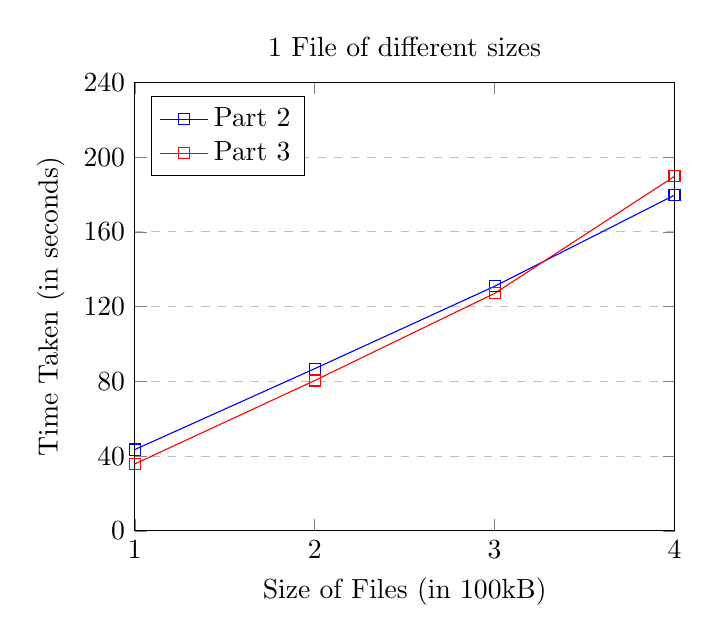
\begin{tikzpicture}
\begin{axis}[
    title={1 File of different sizes},
    xlabel={Size of Files (in 100kB)},
    ylabel={Time Taken (in seconds)},
    xmin=1, xmax=4,
    ymin=0, ymax=240,
    xtick={1,2,3,4},
    ytick={0,40,80,120,160,200,240},
    legend pos=north west,
    ymajorgrids=true,
    grid style=dashed,
]

\addplot[
    color=blue,
    mark=square,
    ]
    coordinates {
    (1, 43.50957600) (2, 86.80219800) (3, 130.90629800) (4, 179.70722000)
    };

\addplot[
    color=red,
    mark=square,
    ]
    coordinates {
    (1, 35.80605200) (2, 80.46090200) (3, 127.08874900) (4, 189.76057300)
    };
    \legend{Part 2, Part 3}
    
\end{axis}
\end{tikzpicture}
\end{multicols}

\pagebreak
\section*{Tokens}
Token Distribution
\begin{itemize}
    \item Om : 10
    \item Sarwagya : 10
    \item Amaiya : 10
\end{itemize}

\begin{center}
\begin{tabular}{ |c|c|c| } 
\hline
 Token No. & Person & Work done \\
 \hline
 1 & Om & Part 1 \\ 
 2 & Om & Creating git repo \\ 
 3 & Amaiya & Creating list.c \\ 
 4 & Amaiya & Testing list.c \\
 5 & Amaiya & Creating hm.c \\ 
 6 & Amaiya & Testing hm.c \\ 
 7 & Sarwagya & Creating mythreads.c \\
 8 & Sarwagya & Creating mythreads.c \\
 9 & Sarwagya & Testing mythreads.c \\
10 & Amaiya &  Testing main.c without threads\\ 
 11 & Amaiya & Testing main.c with threads without yield \\ 
 12 & Sarwagya & Implementing mythread\textunderscore yield \\ 
 13 & Sarwagya & Implementing locks \\
14 &  Sarwagya & Testing main.c with yield \\ 
 15 & Sarwagya & Testing main. with locks \\ 
 16 & Sarwagya & Creating make file for Part 2 \\ 
 17 & Sarwagya & Creating make file for Part 3 \\ 
  18 & Om & Running Part 2 code with large files \\ 
 19 & Om & Running Part 3 code with large files\\ 
 20 & Om & Debugging segfaults for large files \\
 21 & Om & Debugging hash function giving negative values \\ 
 22 & Sarwagya &  Uploading final code on git\\  
 23 & Om & Collected data for graphs and tables\\
 24 & Om & Double checked all functions with submission guidelines\\
 25 & Amaiya & Writing report in latex \\ 
 26 & Amaiya & Plotting graphs in latex \\ 
 27 & Amaiya &  Making tables in latex \\
28 & Amaiya & Checked and reviewed final code \\ 
 29 & Om & Writing comments for Doxygen \\ 
 30 & Om & Creating the doxygen file \\
 
 
 \hline
\end{tabular}
\end{center}

\end{document}
